\documentclass[10.5pt,a4paper]{article}
% NeonArch — final report, IC-6600 II Programmed Project (Alternative A)
% Build: latexmk -pdf main.tex   (figures: python3 make_figures.py)
\usepackage[utf8]{inputenc}
\usepackage[T1]{fontenc}
\usepackage{mathptmx}
\usepackage[scaled=0.92]{helvet}
\usepackage{courier}
\usepackage[margin=2.2cm]{geometry}
\usepackage{graphicx}
\usepackage{booktabs}
\usepackage{tabularx}
\usepackage{array}
\usepackage{enumitem}
\usepackage[table]{xcolor}
\usepackage{caption}
\usepackage{float}
\usepackage{fancyhdr}
\usepackage[hidelinks]{hyperref}
\usepackage{xurl}

\definecolor{neon}{HTML}{2A78D6}
\definecolor{pending}{HTML}{FFF4D6}
\definecolor{muted}{HTML}{52514E}
\setlist{itemsep=1pt,topsep=3pt}
\captionsetup{font=small,labelfont=bf}
\setlength{\parskip}{3pt}
\setlength{\emergencystretch}{3em}
\tolerance=2000
\renewcommand{\arraystretch}{1.15}
\newcolumntype{L}{>{\raggedright\arraybackslash}X}
\newcommand{\cmd}[1]{\texttt{#1}}
\newcommand{\pendingbox}[1]{\par\noindent\colorbox{pending}{\parbox{\dimexpr\linewidth-2\fboxsep}{\small\textbf{Pending:} #1}}\par}

\pagestyle{fancy}
\fancyhf{}
\lhead{\small\color{muted}NeonArch — Final report}
\rhead{\small\color{muted}IC-6600 · II Semester 2026}
\cfoot{\small\thepage}
\renewcommand{\headrulewidth}{0.3pt}

\begin{document}

% ------------------------------------------------------------------ title
\begin{titlepage}
\centering
\vspace*{1.5cm}
{\large Instituto Tecnológico de Costa Rica\\ Escuela de Ingeniería en Computación\par}
\vspace{0.6cm}
{\normalsize IC-6600 Principios de Sistemas Operativos\\ II Proyecto Programado · Alternativa A\par}
\vspace{2.2cm}
{\Huge\bfseries\color{neon} NeonArch\par}
\vspace{0.3cm}
{\Large A custom Linux distribution on Arch Linux,\\ built, instrumented and measured\par}
\vspace{2.2cm}
{\large Final report\par}
\vspace{1.8cm}
\begin{tabular}{ll}
Hernán Alonso Gutiérrez Quesada & 2023-800-185\\
Royner Baltodano Sánchez & \textit{carné}\\
\end{tabular}
\vspace{1.4cm}

{Professor: Jorge Alberto Alfaro Velasco\par}
\vfill
{Repository: \url{https://github.com/Hernan1787/neonarch}\par}
\vspace{0.3cm}
{November 2026\par}
\end{titlepage}

% ------------------------------------------------------------------ abstract
\section*{Summary}
NeonArch is not a downloadable image: it is a reproducible layer of configuration, scripts, systemd units, pacman hooks and own commands applied by an idempotent bootstrap (\cmd{install.sh}) on top of an Arch Linux system that each member installed by hand (UEFI, btrfs with subvolumes, systemd-boot). Seven operating-system topics were implemented and \emph{measured}; this report integrates the technical decisions, the measurements, the limitations we found and the lessons learned. Several results contradicted our first expectations (an ``optimisation'' that made the boot slower, a benchmark that was measuring RAM instead of the disk, a scheduler behaviour that changed in recent kernels); in every case we kept the data and explained it rather than discarding it.

\vspace{4pt}
\noindent\begin{tabularx}{\linewidth}{@{}lL@{}}
\toprule
\textbf{Environment} & \textbf{Value}\\ \midrule
Host & AMD Ryzen 5 3600X (6C/12T), 16 GB RAM, NVMe SSD, Windows 11, VirtualBox 7.2\\
VM & 2 vCPU, 4 GiB RAM, 40 GiB VDI, UEFI (OVMF), VMSVGA without 3D, NAT\\
OS & Arch Linux, kernel 7.2.15-arch1-1, systemd 262, pacman 7.1.0, btrfs root\\
Desktop & i3 window manager on X11, xterm, rofi, i3status, dunst (``Neon'' theme)\\
\bottomrule
\end{tabularx}

\tableofcontents
\newpage

% ================================================================== 1
\section{Layer 1 — Base installation and reproducibility}

\subsection{Manual installation decisions}
Each member installed Arch by hand following \cmd{docs/instalacion.md}, which explains \emph{why} each command is run (\cmd{archinstall} was not used). Table~\ref{tab:install} summarises the decisions that later topics depend on.

\begin{table}[H]
\centering\small
\begin{tabularx}{\linewidth}{@{}>{\raggedright\arraybackslash}p{0.36\linewidth}L@{}}
\toprule
Decision & Reason\\ \midrule
UEFI + GPT, 1 GiB FAT32 ESP & Required by the assignment; the firmware reads EFI executables only from a FAT ESP. 1 GiB holds several kernels/initramfs (systemd-boot loads them from the ESP).\\
btrfs root with subvolumes \cmd{@ @home @snapshots @var\_log @pkg @swap} & Topic 3. A snapshot of \cmd{@} excludes user files, logs, package cache and swap, so a rollback restores the system without losing data or the logs that explain what broke.\\
Mount options \cmd{noatime}, \cmd{compress=zstd:1}, \cmd{space\_cache=v2}; \cmd{subvol=} only, no \cmd{subvolid=} & Avoid a CoW metadata write on every read; transparent compression; a rolled-back \cmd{@} has a new ID, so pinning the ID would break the boot.\\
systemd-boot & Plain-text entries; easy to add kernel parameters and rescue entries (Topic 7).\\
ESP mounted \cmd{fmask=0077,dmask=0077} & Only root can read the bootloader files (Topic 9).\\
Normal user in \cmd{wheel} + sudo & Least privilege; every privileged action is logged.\\
\bottomrule
\end{tabularx}
\caption{Installation decisions (details and the reason for every command: \cmd{docs/instalacion.md}).}
\label{tab:install}
\end{table}

\textbf{Problems found.} The installation log records 14 real problems with cause and fix: virtualisation (AMD-V/SVM) disabled in the BIOS — it was disabled again later by a firmware reset —, typos that created no subvolume or a wrong kernel parameter (\cmd{rm} instead of \cmd{rw}), a \cmd{sed} expression without the file separator that silently generated no locale, a \cmd{loader.conf} written to the wrong path, the bootloader not registering its NVRAM entry from inside \cmd{arch-chroot} (fixed after the first boot with \cmd{bootctl install}), and two problems of the desktop described below. Current Arch no longer builds the \emph{fallback} initramfs, so the guide was corrected to create a single boot entry.

\subsection{Idempotent bootstrap}
\cmd{install.sh} turns a clean manual install into NeonArch in six stages; each stage first compares the current state with the desired one and acts only if they differ (Table~\ref{tab:bootstrap}). Every run writes a log to \cmd{logs/}. On \cmd{neonarch-hernan} the first full run applied 21 changes and the next run reported \emph{``system already up to date: 0 changes (idempotent run)''} (\cmd{logs/install-neonarch-hernan-20261110-231929.log}).

\begin{table}[H]
\centering\small
\begin{tabularx}{\linewidth}{@{}l>{\raggedright\arraybackslash}p{0.42\linewidth}L@{}}
\toprule
Stage & Action & Idempotency check\\ \midrule
packages & install \cmd{pkglist.txt} (+ VM guest tools by \cmd{systemd-detect-virt}) & \cmd{pacman -T} lists only unsatisfied packages\\
dotfiles, commands & symlink \cmd{dotfiles/*} into \cmd{\$HOME}, \cmd{bin/*} into \cmd{\textasciitilde/.local/bin} & skip links that already point to the repo; back up real files\\
system & copy units, hooks, udev rules, sysctl, zram, helper scripts, sudoers drop-ins (validated with \cmd{visudo -c} first) & \cmd{cmp} with the installed copy; \cmd{daemon-reload} only if a unit changed\\
services & enable units of \cmd{config/services.txt} & \cmd{systemctl is-enabled}\\
snapper & create the snapshot configuration & \cmd{snapper get-config}\\
\bottomrule
\end{tabularx}
\caption{Stages of \cmd{install.sh}.}
\label{tab:bootstrap}
\end{table}

\subsection{Desktop: i3, justified with data}
i3 was compared with XFCE 4.20 installed temporarily. Both sessions were started identically (fresh boot, tty1 login, \cmd{startx}; the session is chosen by \cmd{\textasciitilde/.config/neonarch/session}) with only one xterm open; \cmd{scripts/measure-desktop.sh} waits 60\,s and takes five samples 10\,s apart.

\begin{figure}[H]
\centering
\begin{minipage}{0.47\linewidth}\centering
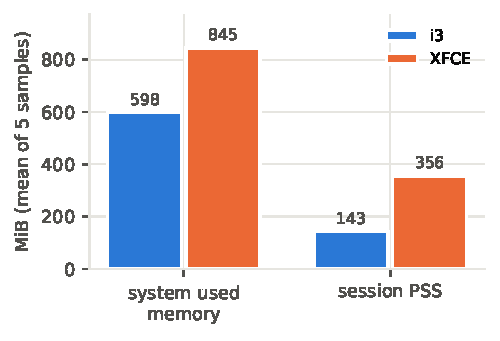
\includegraphics[width=\linewidth]{figures/desktop.pdf}
\end{minipage}\hfill
\begin{minipage}{0.5\linewidth}\small
\begin{tabular}{@{}lrr@{}}
\toprule
 & i3 & XFCE\\ \midrule
Used memory (MiB) & 598 & 845\\
User processes & 25 & 41\\
User RSS (MiB) & 245 & 776\\
User PSS (MiB) & 143 & 356\\
\bottomrule
\end{tabular}
\end{minipage}
\caption{Idle desktop footprint (mean of 5 samples; \cmd{docs/evidence/desktop/}).}
\end{figure}

XFCE adds 16 always-running processes (session manager, \cmd{xfdesktop}, \cmd{xfsettingsd}, \cmd{xfconfd}, panel and plugins, Thunar daemon, power manager, polkit agent, accessibility bus) and 2.5$\times$ the session's proportional memory. PSS is the fair metric because RSS counts shared GTK libraries once per process. Two measurement artefacts were identified and excluded in the discussion: the Alt+F2 launcher left running (42\,MB) and a VirtualBox guest helper that grew to 112\,MB only in the XFCE session. Even without them XFCE uses about 2.5$\times$ the RSS of i3. A lower baseline matters because Topic~2 creates memory pressure on a 4\,GiB VM.

\textbf{Terminal.} Alacritty (GPU-rendered) hung without drawing a window: VirtualBox's VMSVGA adapter has no 3D support. Every \emph{Super+Enter} left a stuck process (21 of them; RAM grew from 178\,MiB to 1.6\,GiB). From tty2 we proved the key arrived (\cmd{showkey}: keycode 125) and replaced the terminal by xterm, rendered on the CPU.

% ================================================================== 2
\section{Layer 2 — Operating-system topics}
Seven of the nine topics were implemented (Table~\ref{tab:topics}). Topics 5 (IPC) and 8 (I/O and devices) were left out: inside a VM the GPU/NPU and hot-plug evidence of Topic 8 would be limited to virtual devices. Each topic has an evidence sheet \cmd{docs/tema-XX-*.md} with the five elements of Annex 2 and the raw data in \cmd{docs/evidence/}.

\begin{table}[H]
\centering\small
\begin{tabular}{@{}llll@{}}
\toprule
Topic & Owner & Main artefacts & Headline result\\ \midrule
1 Processes & Hernán & \cmd{neon-ps}, \cmd{tema01-experiment.py} & shares 69.8/22.8/7.4\,\% vs 69.7/22.8/7.5\,\%\\
2 Memory & Royner & zram + swapfile, \cmd{neon-mem} & \textit{pending}\\
3 Filesystem & Hernán & snapper, snap-pac, fio, rollback demo & writes 3.2–3.8$\times$ slower on CoW\\
4 Services & Hernán & \cmd{neon-health.service} + timer & quota 20\,\% $\rightarrow$ 19.8\,\% measured\\
6 Packages & Hernán & ALPM hook, \cmd{neonarch-tools} PKGBUILD & hook in every transaction\\
7 Boot & Hernán & boot measurement, 2 optimisations, rescue & lz4 +10\,\% slower; defaults kept\\
9 Security & Royner & nftables, SSH, sudoers, ACL & \textit{pending}\\
\bottomrule
\end{tabular}
\caption{Implemented topics.}
\label{tab:topics}
\end{table}

% ------------------------------------------------------------------ T1
\subsection{Topic 1 — Processes and scheduling}
\textbf{Implementation.} \cmd{neon-ps} lists PID, PPID, state, nice, policy, real-time priority, last CPU and \%CPU (two samples of \cmd{utime+stime} from \cmd{/proc/<pid>/stat}) and changes nice (\cmd{setpriority}), policy (\cmd{sched\_setscheduler}) and affinity (\cmd{sched\_setaffinity}). \cmd{neon-boost} raises the nice value and I/O priority of every thread of a process (\cmd{/proc/<pid>/task}, \cmd{ioprio\_set}).

\textbf{Concept.} Linux 7.2 uses EEVDF for the fair class: each task's virtual runtime advances inversely to its weight (nice 0 = 1024, each step $\approx\times1.25$) and, among eligible tasks, the one with the earliest virtual deadline runs. Real-time classes always preempt the fair class.

\textbf{Method.} Three CPU-bound loops pinned to CPU~0 with nice 0, 5, 10; then a \cmd{SCHED\_FIFO} loop (priority 10) against a normal one; 3 runs of 20\,s, CPU time read from \cmd{/proc}.

\begin{figure}[H]
\centering
\begin{minipage}{0.47\linewidth}\centering
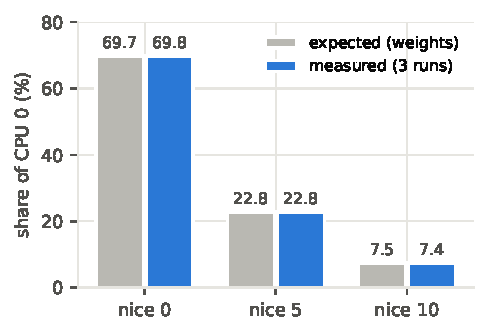
\includegraphics[width=\linewidth]{figures/t1-nice-shares.pdf}
\end{minipage}\hfill
\begin{minipage}{0.5\linewidth}\small
\begin{tabular}{@{}lrr@{}}
\toprule
SCHED\_FIFO vs SCHED\_OTHER & FIFO & OTHER\\ \midrule
run 1 & 94.10\,\% & 4.98\,\%\\
run 2 & 94.00\,\% & 5.05\,\%\\
run 3 & 93.99\,\% & 5.04\,\%\\
\bottomrule
\end{tabular}
\end{minipage}
\caption{Left: share of one core by nice value. Right: real-time vs fair class on one core.}
\end{figure}

\textbf{Interpretation.} The fair shares match $w_i/\sum w$ to $\pm$0.1 percentage points: nice does not give absolute priority but a proportional share, and nice 10 is never starved. In the second experiment the FIFO task dominates, yet the normal task received exactly 5\,\%. On this kernel \cmd{sched\_rt\_runtime\_us} equals the period (classic RT throttling disabled); the 5\,\% comes from the \emph{fair server}, a deadline server that reserves 50\,ms per second for fair tasks on each CPU. We verified it in \cmd{/sys/kernel/debug/sched/fair\_server/cpu0}: runtime 50\,000\,000\,ns, period 1\,000\,000\,000\,ns. Our script's ``expected $\leq$95\,\%'' column assumed the old mechanism, which the measurement corrected.

% ------------------------------------------------------------------ T2
\subsection{Topic 2 — Memory}
\textbf{Implementation.} zram (\cmd{zram-generator}: 50\,\% of RAM, zstd, priority 100) and a 2\,GiB NOCOW swapfile on \cmd{@swap} (priority 10): the kernel uses the highest priority first, so pages go to compressed RAM (microseconds) before the disk (milliseconds). VM tuning for zram (\cmd{vm.swappiness=180}, \cmd{vm.page-cluster=0}). Real-time monitor \cmd{neon-mem}: RAM, swap devices and priorities, zram compression ratio, swap-in/out and major faults per second, top processes by page faults.

\textbf{Method.} \cmd{stress-ng --vm} allocating MemAvailable + 1.5\,GiB for 60\,s, with and without zram; \cmd{vmstat} \cmd{si/so}, deltas of \cmd{pswpin}/\cmd{pswpout}/\cmd{pgmajfault}, zram \cmd{mm\_stat}, throughput and OOM-killer messages.

\pendingbox{results and interpretation from \cmd{scripts/tema02-measure.sh} on Royner's VM (\cmd{docs/tema-02-memoria.md}).}

% ------------------------------------------------------------------ T3
\subsection{Topic 3 — Filesystem (btrfs)}
\textbf{Implementation.} btrfs root with the subvolume layout of Table~\ref{tab:install}; snapper with hourly timeline snapshots (5 hourly + 7 daily kept) and \cmd{snap-pac}, which takes a \emph{pre} and a \emph{post} snapshot around every pacman transaction; shortcut \emph{Super+Shift+S} for a manual snapshot.

\textbf{Method.} fio with \cmd{O\_DIRECT}, \cmd{io\_uring}, depth 16, 1\,GiB, 3 runs of 20\,s per workload. The ext4 reference is a loop image \emph{on the same btrfs root} created NOCOW (\cmd{chattr +C}) and attached with \cmd{losetup --direct-io=on}.

\begin{figure}[H]
\centering
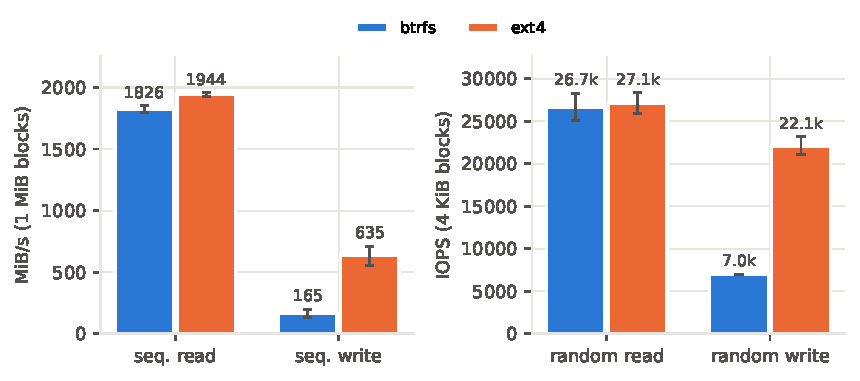
\includegraphics[width=0.92\linewidth]{figures/t3-fio.pdf}
\caption{btrfs (CoW, zstd:1) vs ext4 on the same virtual disk (mean $\pm$ sd of 3 runs).}
\end{figure}

\textbf{Interpretation.} Reads are equivalent (within 2–6\,\%): reading changes nothing, so copy-on-write costs nothing. Writes are 3.8$\times$ (sequential) and 3.2$\times$ (random, 2.29 vs 0.72\,ms per I/O) slower on btrfs: every write allocates a new extent, stores a checksum and updates the B-trees up to the root, and metadata is duplicated (\cmd{DUP}). The NOCOW image sits on the same filesystem and device and writes 3–4$\times$ faster, which isolates CoW as the cause. We still chose btrfs because a desktop is read-dominated and CoW gives snapshots, rollback and checksums; write-heavy files (swap, VM images) belong in NOCOW subvolumes, as we did with \cmd{@swap}.

\textbf{Discarded measurement.} The first run gave ext4 5\,785\,MiB/s and 217\,914 random-read IOPS (71\,µs): impossible for this disk. The loop device was buffered, so ext4 was reading the host's page cache. The data were kept (\cmd{fio/discarded-buffered-loop/}) and the benchmark was repeated with a direct-I/O loop.

\textbf{Rollback demo.} Removing \cmd{htop} with pacman created snapshots \#22 (pre) and \#23 (post). \cmd{snapper status 22..23} showed the deleted binary, man page, icons \emph{and pacman's database entry}; \cmd{snapper undochange 22..23} restored them (\cmd{create:9 modify:2}) and \cmd{pacman -Q htop} recognised the package again. \cmd{pacman -Qkk} then reported 5 files with only a modification-time mismatch: \cmd{undochange} is a file-level copy. An exact whole-system rollback is \cmd{snapper rollback} (switching the default subvolume).

% ------------------------------------------------------------------ T4
\subsection{Topic 4 — Service management (systemd)}
\textbf{Implementation.} \cmd{neon-health.service}: a daemon that samples \cmd{/proc} every 10\,s into its state directory, with \cmd{After=local-fs.target}, \cmd{Wants=} a report timer (hourly, \cmd{Persistent=true}), \cmd{Restart=on-failure} with a start-rate limit, \cmd{CPUQuota=20\%}, \cmd{MemoryMax=64M}, \cmd{MemorySwapMax=0}, and sandboxing (\cmd{DynamicUser}, \cmd{ProtectSystem=strict}, \cmd{ProtectHome}, \cmd{NoNewPrivileges}). Signals \cmd{SIGUSR1}/\cmd{SIGUSR2} trigger a CPU burn and an unbounded allocation to test the limits.

\begin{figure}[H]
\centering
\begin{minipage}{0.47\linewidth}\centering
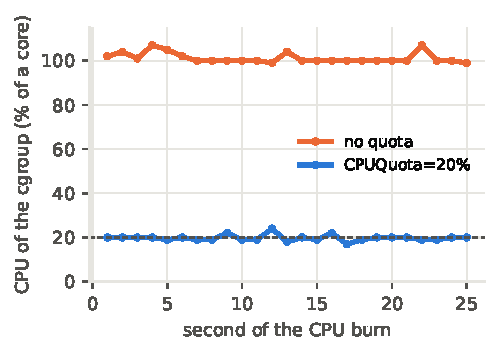
\includegraphics[width=\linewidth]{figures/t4-cpuquota.pdf}
\end{minipage}\hfill
\begin{minipage}{0.5\linewidth}\small
\begin{tabularx}{\linewidth}{@{}Lr@{}}
\toprule
Test & Result\\ \midrule
CPU burn, \cmd{CPUQuota=20\%} & 19.8\,\%\\
CPU burn, quota removed & 101.2\,\%\\
allocate beyond 64\,MiB & OOM kill, restart (0$\rightarrow$1)\\
\cmd{SIGKILL} & restart (1$\rightarrow$2)\\
\bottomrule
\end{tabularx}
\end{minipage}
\caption{CPU of the service's cgroup (\cmd{cpu.stat} sampled every second) and failure tests.}
\end{figure}

\textbf{Interpretation.} systemd places each service in its own cgroup~v2. \cmd{CPUQuota=20\%} becomes \cmd{cpu.max = 20000 100000}: the group may run 20\,ms per 100\,ms period and is then throttled. This is a hard cap, unlike nice, which only shares the CPU when there is contention. \cmd{MemoryMax} is enforced by the memory controller: the OOM killer acted \emph{inside} the cgroup only, and \cmd{Restart=on-failure} brought the service back. The service never runs as root.

% ------------------------------------------------------------------ T6
\subsection{Topic 6 — Package management (pacman)}
\textbf{Implementation.} An own ALPM hook (\cmd{PostTransaction}, \cmd{NeedsTargets}) logs every transaction, lists orphan packages and warns when the running kernel or systemd were upgraded. The PKGBUILD \cmd{neonarch-tools} packages our five commands with \cmd{makepkg}.

\textbf{Results.} pacman 7.1.0 with \cmd{SigLevel = Required DatabaseOptional} and 183 trusted keys; the local database holds 416 packages, one directory each (\cmd{desc}, \cmd{files}, \cmd{mtree}). Our package: version 1.0.0-2, 11 files, \cmd{pacman -Qo /usr/bin/neon-info} reports ownership and \cmd{pacman -Qkk} reports 0 altered files. In every transaction the order was: snap-pac pre-snapshot $\rightarrow$ package changes $\rightarrow$ our hook $\rightarrow$ snap-pac post-snapshot. \cmd{pacman -Sp xfce4-terminal} resolved 9 dependencies without installing anything.

\textbf{Interpretation and a lesson.} Packaging gives what copying files cannot: ownership (\cmd{-Qo}), integrity checks against the MTREE (\cmd{-Qkk}), upgrades and clean removal. The hook order makes every transaction reversible (Topic~3). The first build packaged four \emph{empty} commands: terminal output had been pasted back into bash, and lines containing \cmd{>} truncated the files. \cmd{pacman -Ql} could not reveal it, but \cmd{tar -tvf} of the package showed 0\,bytes. We restored the files from Git, rebuilt (\cmd{pkgrel=2}) and disabled xterm's copy-on-select.

% ------------------------------------------------------------------ T7
\subsection{Topic 7 — Boot process}
\textbf{Boot chain.} UEFI firmware (NVRAM entry \emph{Linux Boot Manager}) $\rightarrow$ \cmd{systemd-bootx64.efi} reads \cmd{loader.conf} and \cmd{neonarch.conf} $\rightarrow$ loads \cmd{vmlinuz-linux} and \cmd{initramfs-linux.img} from the ESP with \cmd{root=UUID=\ldots{} rootflags=subvol=@ rw} $\rightarrow$ the kernel unpacks the initramfs (systemd-based, mkinitcpio hooks) $\rightarrow$ udev loads the disk and btrfs drivers, the root is mounted and \cmd{switch\_root} runs $\rightarrow$ systemd (PID~1) reaches \cmd{graphical.target} $\rightarrow$ getty $\rightarrow$ login $\rightarrow$ \cmd{startx} $\rightarrow$ i3.

\textbf{Method.} \cmd{systemd-analyze time}, \cmd{blame}, \cmd{critical-chain} and \cmd{plot} after each boot, 3 boots per variant. Two optimisations of the initramfs were tried: lz4 compression (faster decompression) without the useless \cmd{fsck} hook (btrfs), and a ``slim'' image (zstd, without \cmd{fsck} and \cmd{kms}).

\begin{figure}[H]
\centering
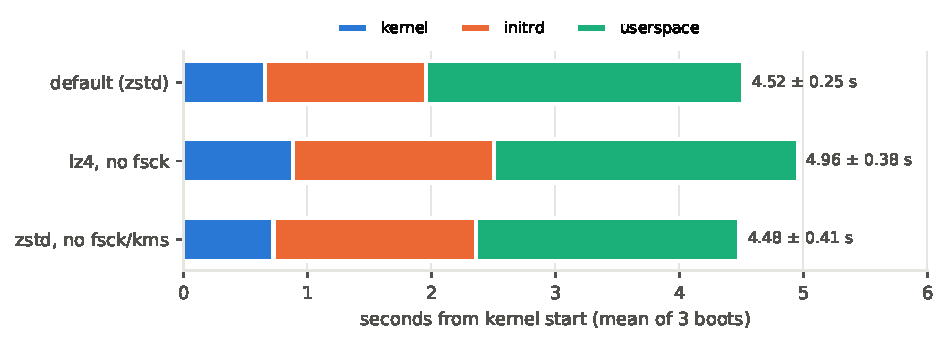
\includegraphics[width=0.92\linewidth]{figures/t7-boot.pdf}
\caption{Boot phases per initramfs variant (mean of 3 boots; total mean $\pm$ sd). Image sizes: 15.2, 21.9 and 14.9\,MB.}
\end{figure}

\textbf{Interpretation.} lz4 made the boot \emph{slower} (+0.55\,s in kernel+initrd, very consistent): its image is 44\,\% larger, and on a Ryzen CPU the extra I/O costs more than the faster decompression saves. The slim image (only 2\,\% smaller) was within the noise of the default. The critical chain is dominated by device discovery (\cmd{.device} units $\approx$1.9\,s in \cmd{blame}), not by the initramfs. We kept the Arch defaults: two plausible optimisations were \emph{rejected with data}. The firmware and loader phases are not reported in this VM (no \cmd{LoaderTime*} EFI variables), so the menu timeout change could not be measured. The first recorded boot (just after a system upgrade, with \cmd{ldconfig} in the critical chain) was discarded.

\textbf{Rescue demo.} Extra boot entries add \cmd{systemd.unit=rescue.target} and \cmd{emergency.target}; \cmd{bootctl set-oneshot} selects one for the next boot only. In rescue, \cmd{sulogin} asks for the root password and only 11 targets are active (sysinit, local-fs, swap, rescue…): filesystems mounted, but no \cmd{basic}, \cmd{network}, \cmd{multi-user} or \cmd{graphical} target. \cmd{systemctl default} continues the normal boot.

% ------------------------------------------------------------------ T9
\subsection{Topic 9 — Protection and security}
\textbf{Implementation.} Users \cmd{operator} (sudo restricted to restarting/inspecting \cmd{neon-health}) and \cmd{guest} (no sudo); shared directory \cmd{/srv/neonlab} (\cmd{root:neonlab}, mode 2770, setgid, ACLs: operator rwx, guest r-x, default ACLs); nftables with input policy \emph{drop} (loopback, established/related, rate-limited ICMP and SSH); SSH with keys only, no root login, \cmd{AllowGroups wheel}; plus the sandboxing of Topic~4 and the root-only ESP.

\textbf{Method.} Positive and \emph{negative} tests (denied writes, denied sudo commands, refused password login, dropped packets in the kernel log) with \cmd{scripts/tema09-tests.sh}; \cmd{nmap} from another machine with and without the firewall.

\pendingbox{results and interpretation on Royner's VM (\cmd{docs/tema-09-seguridad.md}).}

% ================================================================== 3
\section{Layer 3 — Own commands and shortcuts}
\begin{table}[H]
\centering\small
\begin{tabularx}{\linewidth}{@{}l>{\raggedright\arraybackslash}p{0.12\linewidth}L@{}}
\toprule
Command & Author & OS interfaces\\ \midrule
\cmd{neon-info} (mandatory) & Hernán & \cmd{/proc/\{meminfo, swaps, cpuinfo, loadavg, uptime, [pid]/stat, self/mounts\}}, \cmd{/sys/\{bus/pci, block/zram*, class/accel, devices/system/cpu, firmware/efi\}}, \cmd{uname}, \cmd{statvfs}, \cmd{sched\_getscheduler}; GPU/NPU with driver from sysfs (\cmd{vmwgfx} here); \cmd{--sources} prints the interface behind each value\\
\cmd{neon-ps} & Hernán & \cmd{/proc/[pid]/stat}, \cmd{setpriority}, \cmd{sched\_setscheduler}, \cmd{sched\_setaffinity}\\
\cmd{neon-boost} & Hernán & \cmd{/proc/[pid]/task}, \cmd{setpriority}, \cmd{ioprio\_set}; restricted sudoers rule\\
\cmd{neon-net} & Hernán & \cmd{/proc/net/dev}, \cmd{/sys/class/net}, \cmd{ioctl(SIOCGIFADDR)}\\
\cmd{neon-mem} & Royner & \cmd{/proc/\{meminfo, swaps, vmstat, [pid]/stat\}}, \cmd{/sys/block/zram*/mm\_stat}\\
\textit{2 more} & Royner & \textit{pending}\\
\bottomrule
\end{tabularx}
\caption{Own commands (also packaged as \cmd{neonarch-tools}, Topic~6).}
\end{table}

\begin{figure}[H]
\centering
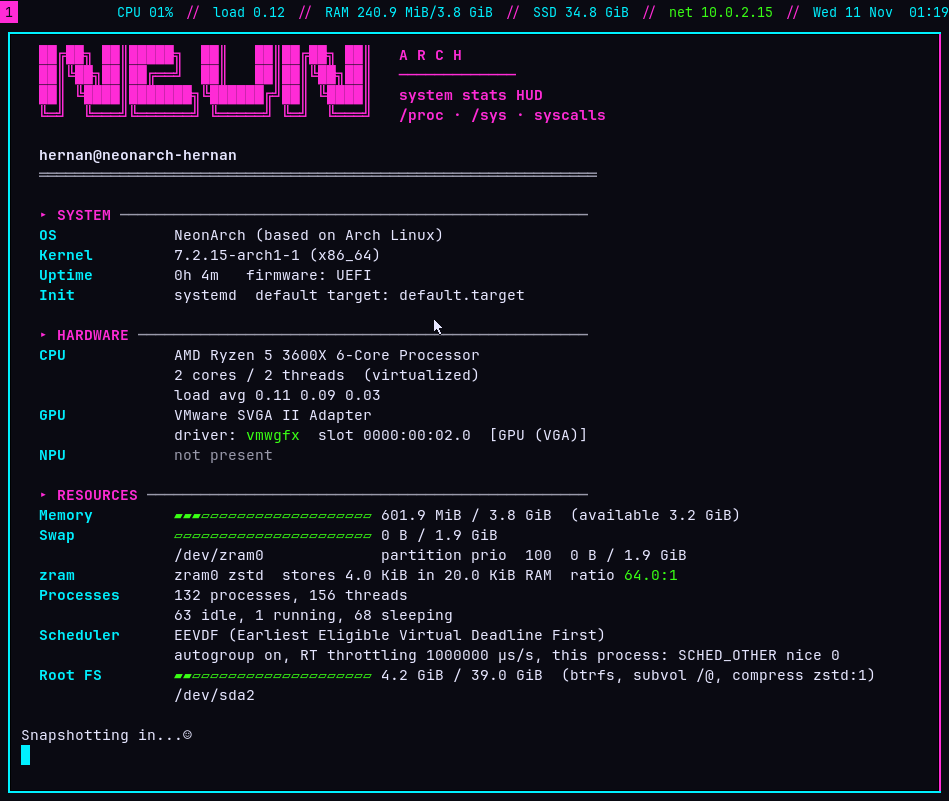
\includegraphics[width=0.62\linewidth]{../img/desktop.png}
\caption{\cmd{neon-info} on \cmd{neonarch-hernan}: every value is read from \cmd{/proc}, \cmd{/sys} or a system call (\cmd{neon-info --sources} prints which). It reports the EEVDF scheduler, the virtual GPU with its driver (\cmd{vmwgfx}), zram and the btrfs root subvolume.}
\end{figure}

Mandatory shortcuts: \emph{Super+Enter} terminal, \emph{Super+W/Q} close, \emph{Super+D} rofi, \emph{Super+1…9} workspaces. Hernán's: \emph{Super+I} \cmd{neon-info} in a floating window, \emph{Super+B} \cmd{neon-boost} on the focused window, \emph{Super+Shift+S} manual btrfs snapshot with a notification. The last one collided with the host: Windows' screenshot shortcut (Win+Shift+S) reached the VM first and created snapshots \#17 and \#19 while we were taking screenshots. Full list: \cmd{docs/cheatsheet.md}.

% ================================================================== 4
\section{Limitations}
\begin{itemize}
\item \textbf{Virtualisation.} All measurements run in VirtualBox over a VDI file. The host's cache and SSD, and the host's own activity, add noise. Boot times varied by up to 0.4\,s between identical boots. Firmware/loader times and real GPU/NPU behaviour are not observable.
\item \textbf{Repetitions.} 3 runs per benchmark and 3 boots per variant are enough to see large effects (CoW writes, lz4) but not small ones (the ``slim'' initramfs).
\item \textbf{Synthetic loads.} fio writes incompressible random data, which removes the benefit of \cmd{compress=zstd}; stress-ng memory pages compress far better than real data.
\item \textbf{Scope.} Topics 5 and 8 were not implemented; the snapper rollback shown is file-level (\cmd{undochange}), not a full subvolume rollback.
\end{itemize}

% ================================================================== 5
\section{Lessons learned}
\begin{itemize}
\item \textbf{Measure, then believe.} Two optimisations that sound right (lz4, slim initramfs) were not, and the scheduler did not follow the textbook RT-throttling model on a 7.x kernel. The data showed it.
\item \textbf{Sanity-check every number against the hardware.} 5.7\,GiB/s from a virtual disk meant we were measuring RAM.
\item \textbf{Verify the artefact, not only its metadata.} The empty package passed \cmd{pacman -Qi}; \cmd{tar -tvf} caught it.
\item \textbf{Know the tool's layer.} bash's command hash made a deleted program look present; xterm's copy-on-select plus pasting output into a shell destroyed files; the host and the guest shared a keyboard shortcut.
\item \textbf{Use of AI.} We used Claude as a tutor and generator of first drafts (\cmd{docs/bitacora\_ia.md}, 8 entries). Five AI errors were detected by measuring or reading the documentation: proposing an ISO that the assignment does not ask for, trailing comments that broke the i3 config, a GPU terminal unusable without 3D, a buffered loop device that biased the benchmark, and the bash-hash problem in the rollback demo. Each one was a lesson about the OS, not only about the tool.
\end{itemize}

\section{Conclusions}
NeonArch is reproducible (manual installation documented step by step, idempotent bootstrap) and every topic is backed by measurements that can be repeated with one script. The measurements confirmed the theory where it applies (proportional fair shares, cgroup limits, the cost of copy-on-write), showed where the theory has moved on (fair server instead of RT throttling), and rejected changes that would only have been assumed to help.

\section*{References}
\small
\begin{itemize}[leftmargin=*]
\item A.~Silberschatz, P.~B.~Galvin, G.~Gagne, \emph{Operating System Concepts}, 10th ed., Wiley, 2018: ch.~2, 3, 5, 9–11, 13–17.
\item Arch Wiki: Installation guide, Btrfs, Snapper, systemd-boot, Mkinitcpio, zram, pacman/Tips, nftables, OpenSSH. \url{https://wiki.archlinux.org}
\item Manual pages: \cmd{sched(7)}, \cmd{systemd.resource-control(5)}, \cmd{systemd.service(5)}, \cmd{bootup(7)}, \cmd{alpm-hooks(5)}, \cmd{PKGBUILD(5)}, \cmd{fio(1)}, \cmd{snapper(8)}, \cmd{proc(5)}.
\item Linux kernel documentation: \emph{EEVDF Scheduler}; \emph{Deadline Task Scheduling} (fair server); \emph{Control Group v2}. \url{https://docs.kernel.org}
\end{itemize}

\end{document}
